\documentclass{article}
\usepackage{float}
\usepackage[pctex32]{graphics}
\usepackage{amssymb}
\usepackage{amsmath}
\usepackage{mathtools}
\usepackage{mathrsfs,relsize}
\usepackage[left=3cm,top=2cm,right=3cm,nohead,nofoot]{geometry}
\usepackage{latexsym}
\usepackage{pstricks}
\usepackage[nottoc]{tocbibind}
\usepackage{hyperref}


\parindent0pt
\parskip6pt
\pagestyle{empty}

\newcommand{\R}{{\mathbb R}}
\newcommand\Laplace{\mathlarger{\mathlarger{\mathscr{L}}}}
\title{Conjugate Gradient Method}
\author{Duttaabhinivesh Devathi}
%content

\begin{document}
\maketitle
\tableofcontents

\section{Problem 1}

\subsection{My Own CGLS Method}

Here it is

\begin{verbatim}

    %%% This is the Conjugate Gradient Least Squares Algorithm, taken from
    %%% Erkki Somersalo's Notes. It solves the normal equations A'*A*x = A'*b.

    function [norms,x] = CGLS(A,b,noise)

        [~,n] = size(A);
        x = zeros(n,1);
        d = b; % Discrepancy Vector, for start, it is b because b - A(0) = b;
        r = A'*b; % residual error A'b - A'Ax = A'(b - Ax) = A'(b - A(0)) = A'b;
        p = r; % Search Directions
        t = A*p; % To save the matrix multiplication so we don't do it again.
        j = 1; % Iteration Variable
        MAXITER = 1000; % Max number of iterations to be safe
        tau = 1.2; % Safety Factor
        norms = zeros(MAXITER,1);
        norms(1) = Inf;

        while(norms(j) > tau*noise && j < MAXITER)

            alpha = (r'*r)/(t'*t);
            x = x + alpha*p;
            d = d - alpha*t;
            rnew = A'*d; % Matrix Multiplication #1
            beta = (rnew'*rnew)/(r'*r);
            p = rnew + beta*p;
            t = A*p; % Matrix Multiplication #2
            r = rnew;
            j = j + 1;
            norms(j) = norm(d);
        end

    end

\end{verbatim}

Let's test it on the Laplace function from Assignment 4.

\begin{equation}
\mbox{\Large\(
\mathscr{L} u(s) = \int_0^{\infty} e^{-st}u(t)dt,   s > 0.
\)}
\end{equation}

Recovering the function $u(t)$ is a challenge if we are given a noisy observation of the Laplace transformation, so we will test CGLS.


\subsection{CGLS Solutions}

We will test our CGLS Method for the Inverse Laplace form

\begin{figure}[H]
    \centerline{
    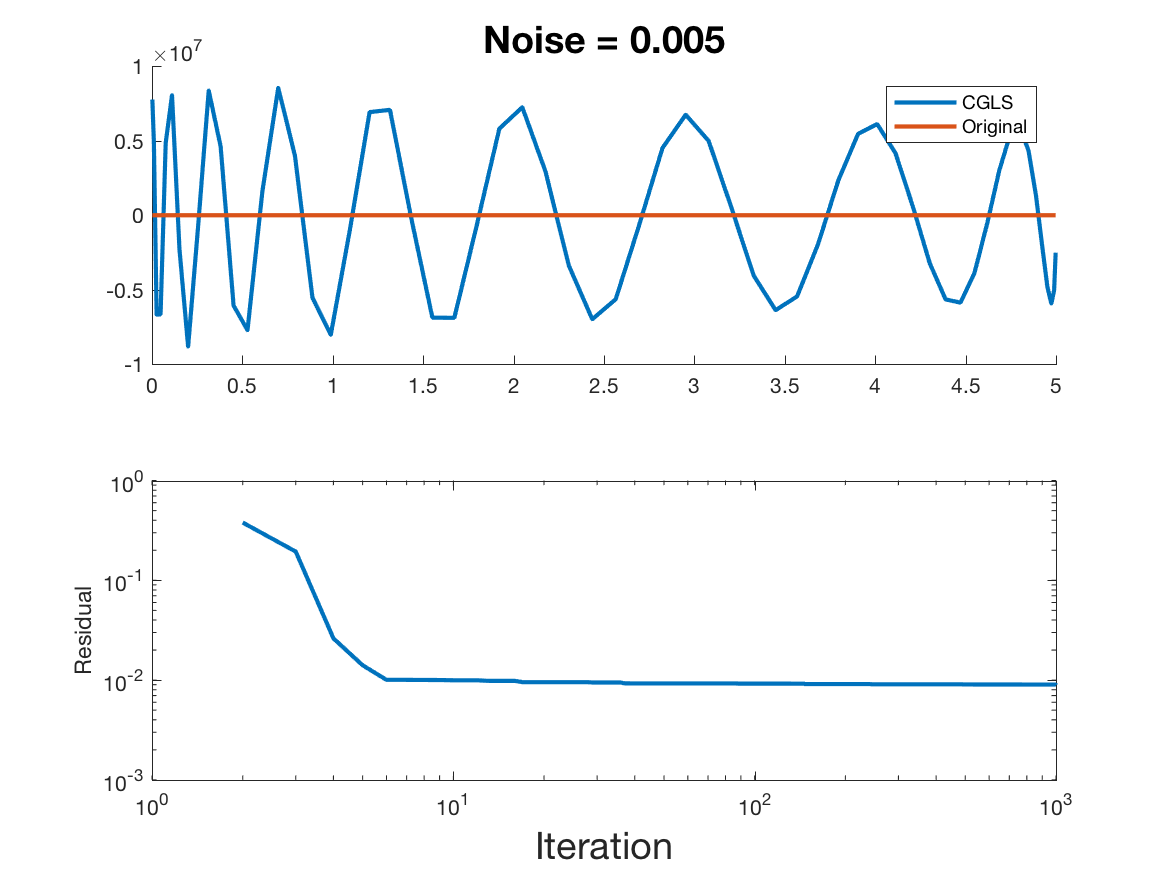
\includegraphics[height = 10 cm]{Laplace_5e-3.png}
    }
    \caption{\label{fig:Laplace_5e-3} Noise = 5*10^{-3}.}
\end{figure}

\begin{figure}[H]
    \centerline{
    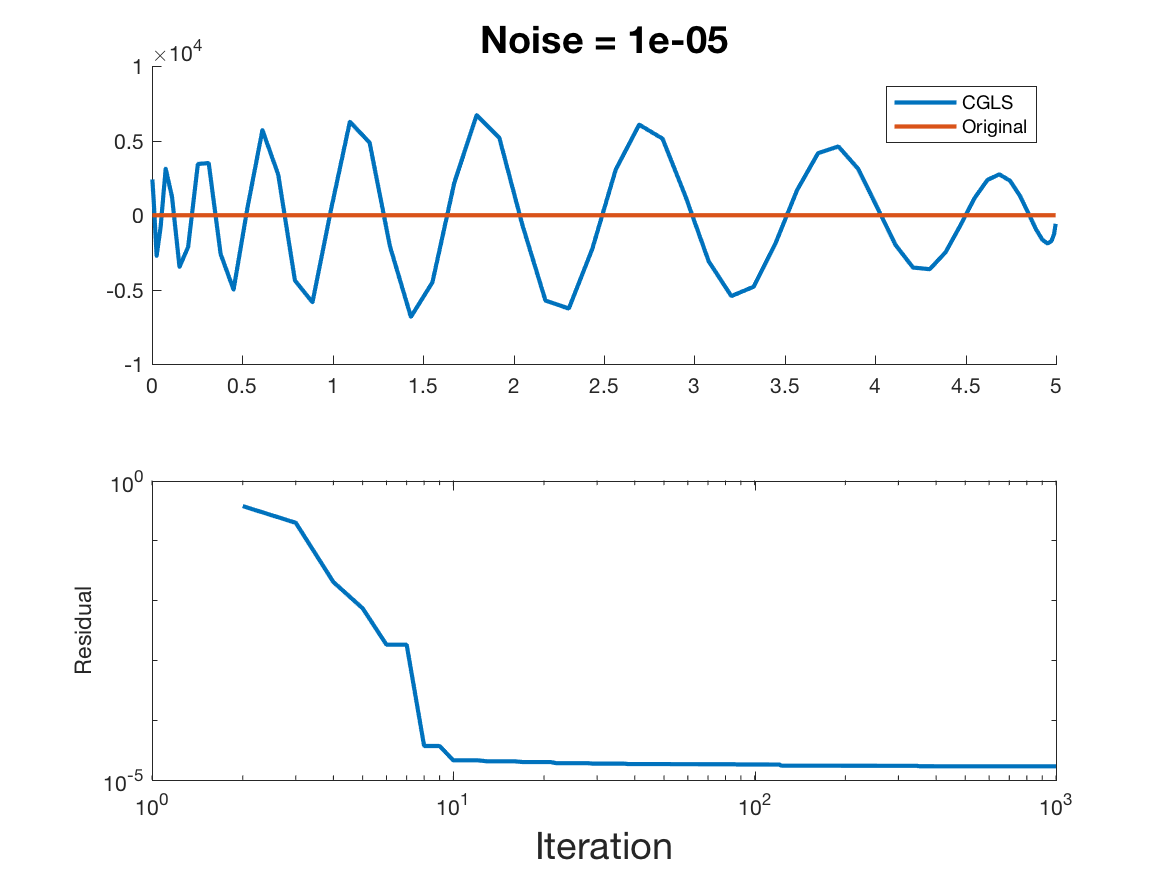
\includegraphics[height = 10 cm]{Laplace_1e-05.png}
    }
    \caption{\label{fig:Laplace_1e-05} Noise = 10^{-5}.}
\end{figure}

\begin{figure}[H]
    \centerline{
    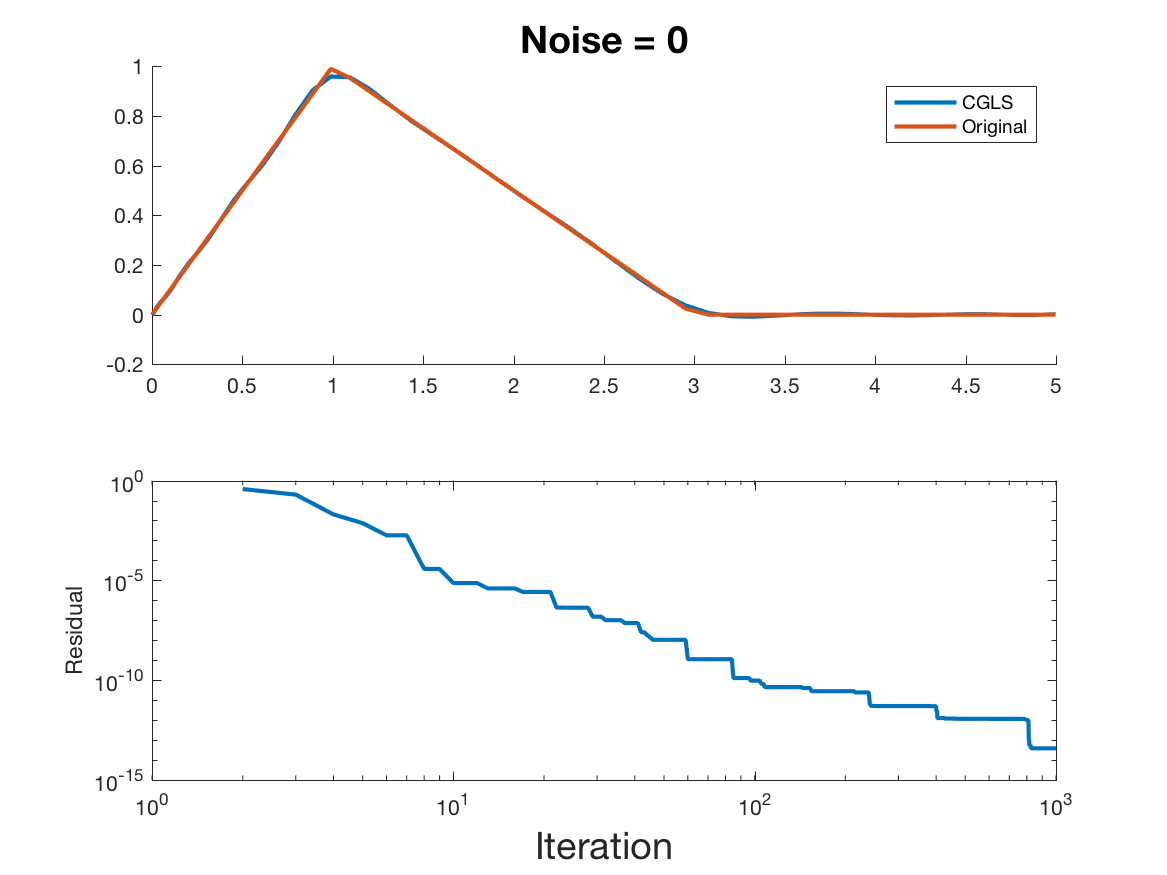
\includegraphics[height = 10 cm]{Laplace_0.png}
    }
    \caption{\label{fig:Laplace_0} Noiseless Solution.}
\end{figure}

It looks like the CGLS Method does not perform well at all if there is any noise in the solution. This could be due to the discretization, which is more dense near 0. Also, the problem is badly conditioned. Look at Figure~\ref{fig:Singular Values}.

\subsection{Singular Values}
Here are the Singular Values of the Normal Equations.

\begin{figure}[H]
    \centerline{
    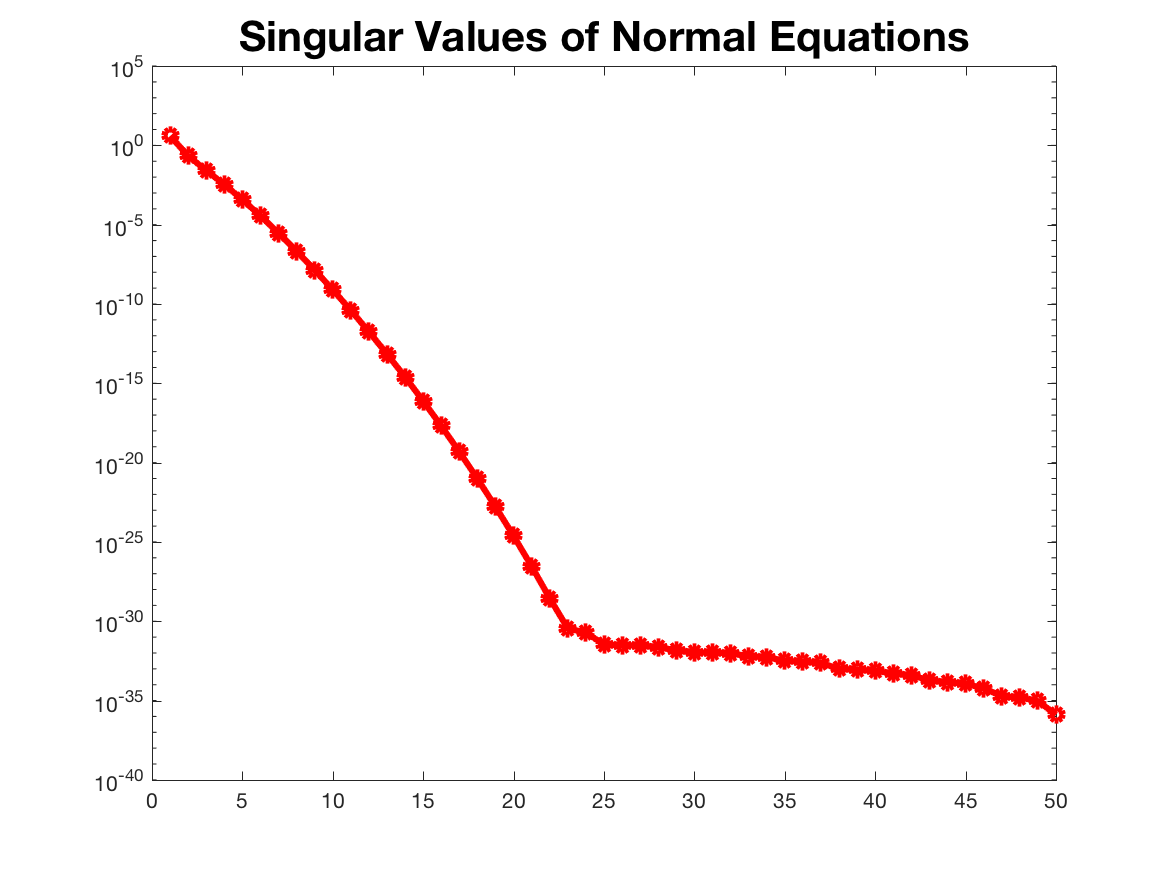
\includegraphics[height = 10 cm]{SingVals.png}
    }
    \caption{\label{fig:Singular Values} The singular values of the forward matrix $A^{T}A$, plotted on a log scale.}
\end{figure}

\section{Problem 2}

This section asks us to do the CGLS on the Backward Heat Equation. To do this, we use \texttt{ode15s} as the forward matrix that propagates $u_{0}$ to $u_{T}$. So we substitute the matrix $A$ with \texttt{ode15s}.

\subsection{Initialization}

This is $u_{0}$:

\begin{figure}[H]
    \centerline{
    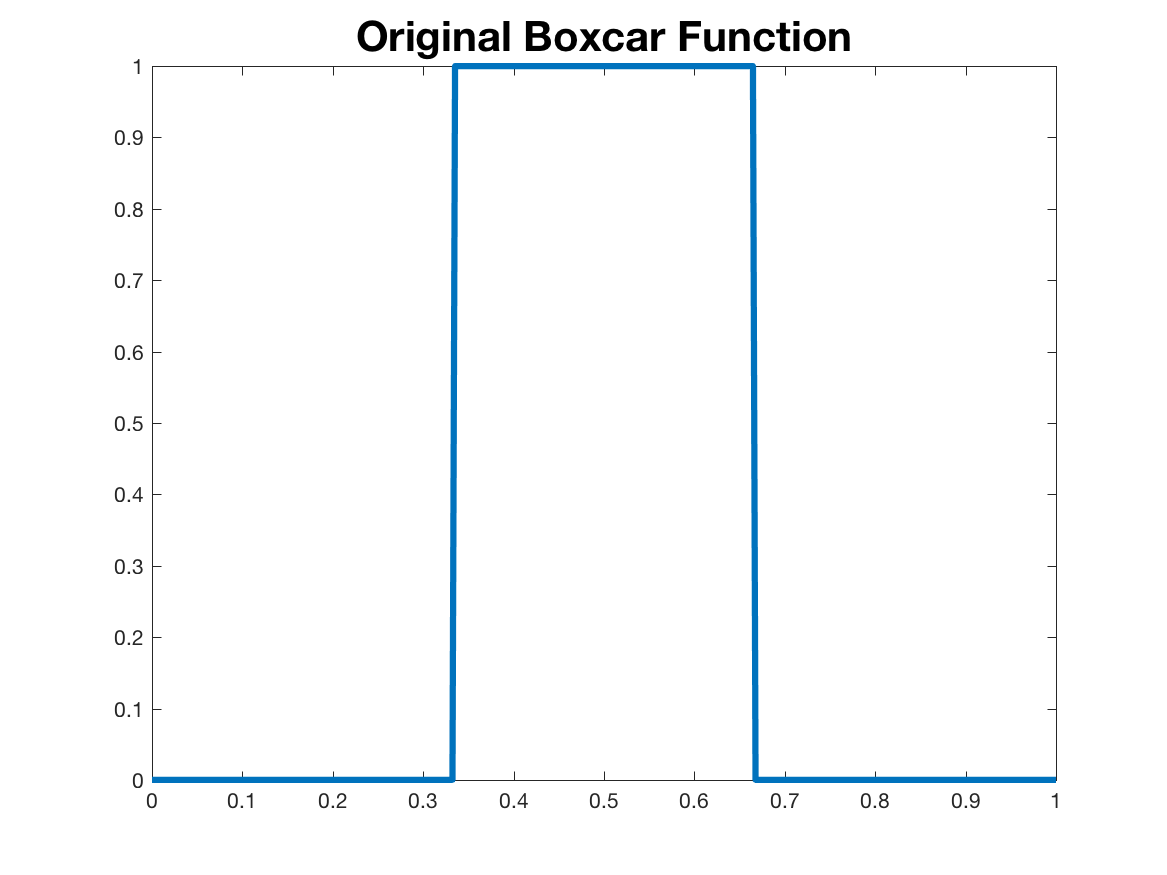
\includegraphics[height = 5 cm]{boxcar.png}
    }
    \caption{\label{fig:boxcar} The original function.}
\end{figure}

Then we add 0.1\% noise to the propagated solution before we solve for $u_{0}$.

This is what we use for $u_{T}$:

\begin{figure}[H]
    \centerline{
    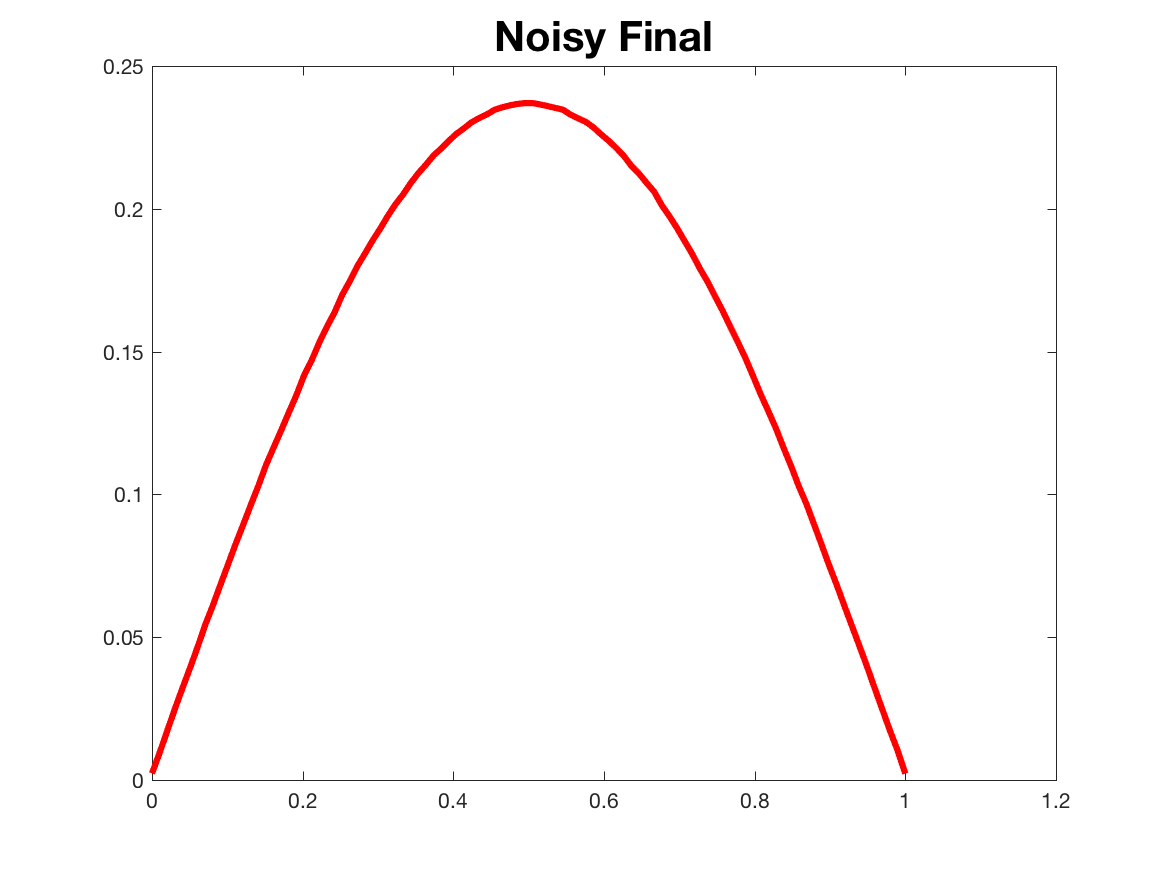
\includegraphics[height = 6 cm]{noisyfinal.png}
    }
    \caption{\label{fig:noisyfinal} The propagated function plus added noise of magnitude $10^{-3}$.}
\end{figure}


\subsection{Finding the Solution}

Now we use CGLS to find the original solution of the Heat Equation based on the Morozov Discrepancy principle.

\begin{figure}[H]
    \centerline{
    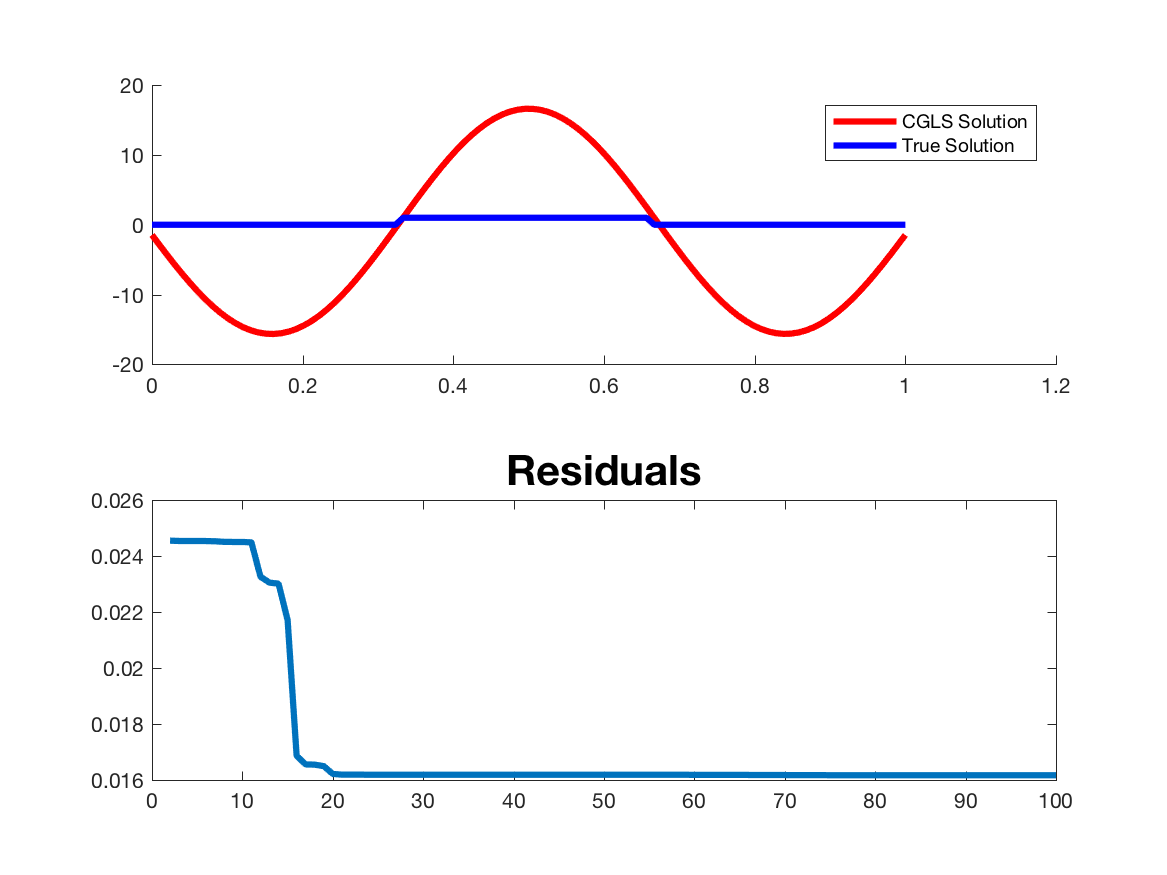
\includegraphics[height = 6 cm]{problem2final.png}
    }
    \caption{\label{fig:problem2final} The propagated function plus added noise of magnitude $10^{-3}$.}
\end{figure}

The CGLS iteration does not perform very well on the reverse heat equation. Perhaps it has to do with the fact that the propagated heat equation only takes on values between 0 and 0.25, or that the \texttt{ode15s} is a badly conditioned problem. Or perhaps, my CGLS method is not good. Let's test it on some more noise levels.

\section{Problem 3}

Here we try the same thing, except we only pick a few points from the original function. To do this, we construct a matrix that picks every k-th point in the $u_{T}$ vector.

In the CGLS Algorithm, this means that we have to do some changes. Namely, when we do ode15s, we have to make sure that the vector inside is the right size. The following snippet of code will show what I mean.

\begin{verbatim}
    alpha = norm(r)^2/norm(t)^2;
    x = x + alpha*p;
    d = d - alpha*t;

    % Here we transform the discrepancy vector to full size before we
    [~,rnew] = ode15s(rhs,tspan,P'*d); rnew = rnew(end,:)'; % This is A'*d
    beta = norm(rnew)^2/norm(r)^2;
    p = rnew + beta*p;

    [~, t] = ode15s(rhs,tspan,p); t = t(end,:)'; % A*p
    t = P*t; % Transform to smaller size
    r = rnew;
    j = j + 1;
    norms(j) = norm(d);
\end{verbatim}

We then try this for different values of k:

\begin{figure}[H]
    \centerline{
    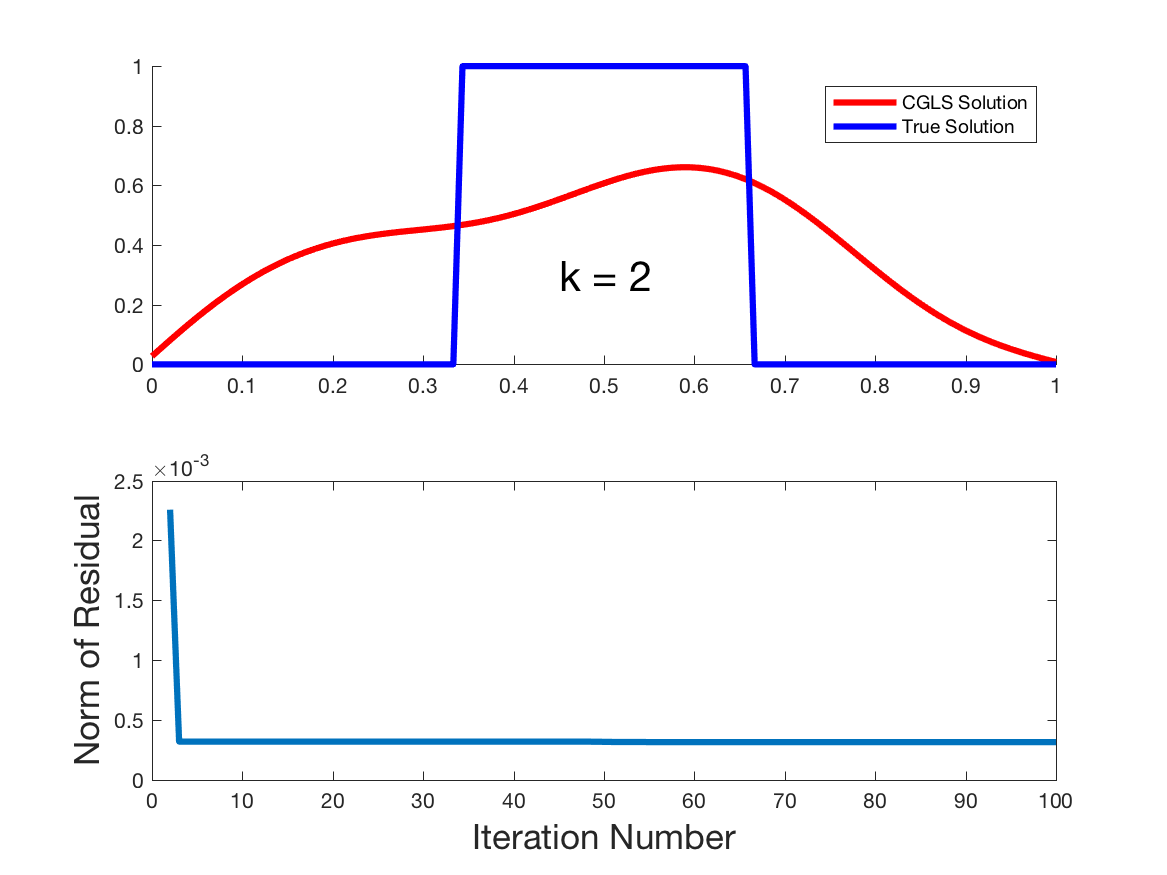
\includegraphics[height = 6 cm]{downsample_k2.png}
    }
    \caption{\label{fig:k2} CGLS Method for Reverse Heat Equation with only picking N/k points from the solution.}
\end{figure}

\begin{figure}[H]
    \centerline{
    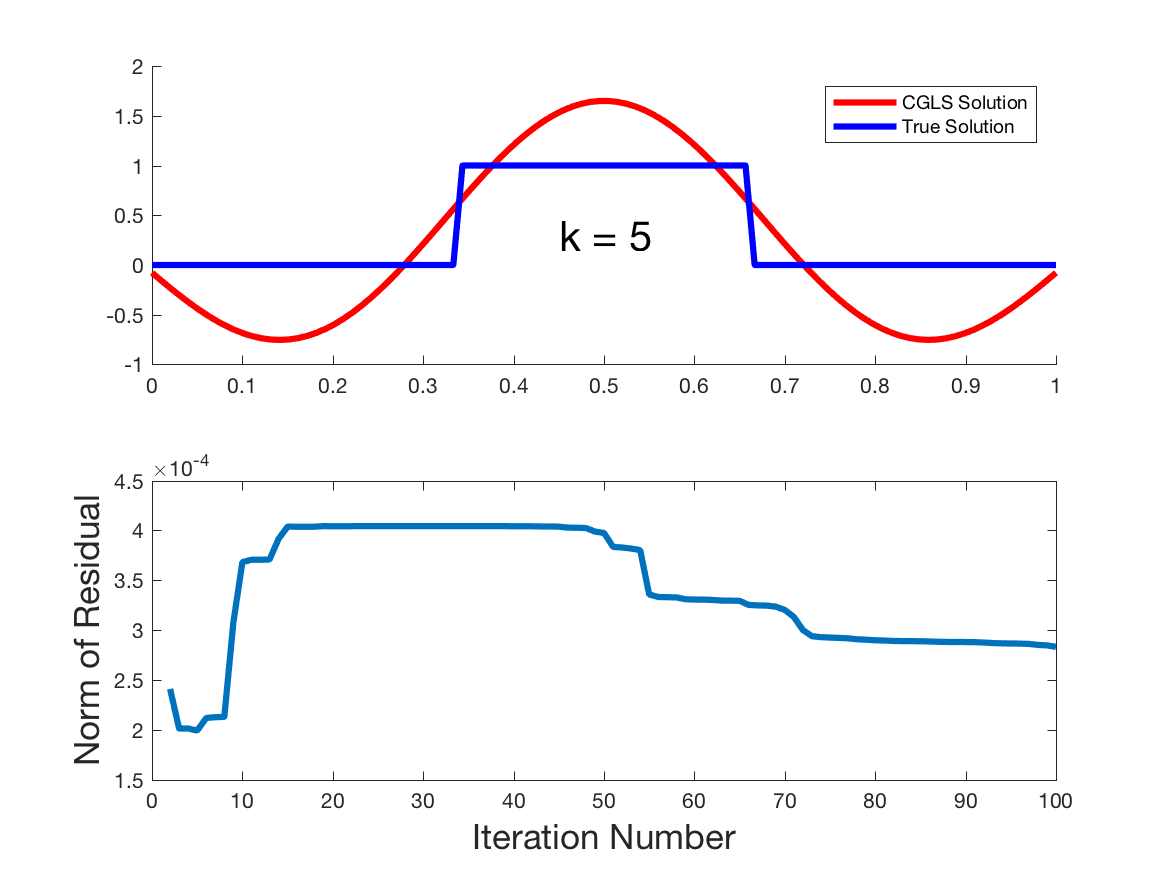
\includegraphics[height = 6 cm]{downsample_k5.png}
    }
    \caption{\label{fig:k5} CGLS Method for Reverse Heat Equation with only picking N/k points from the solution.}
\end{figure}

\begin{figure}[H]
    \centerline{
    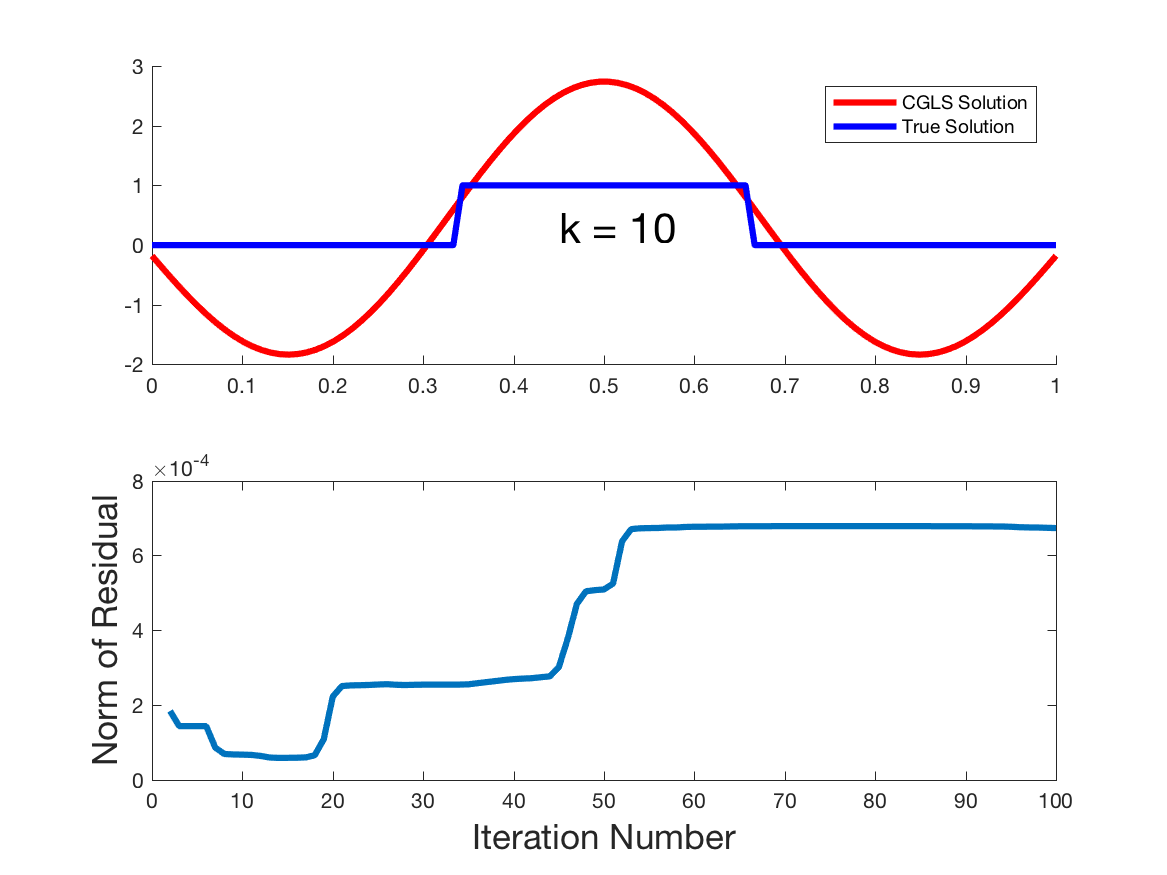
\includegraphics[height = 6 cm]{downsample_k10.png}
    }
    \caption{\label{fig:k10} CGLS Method for Reverse Heat Equation with only picking N/k points from the solution.}
\end{figure}

\begin{figure}[H]
    \centerline{
    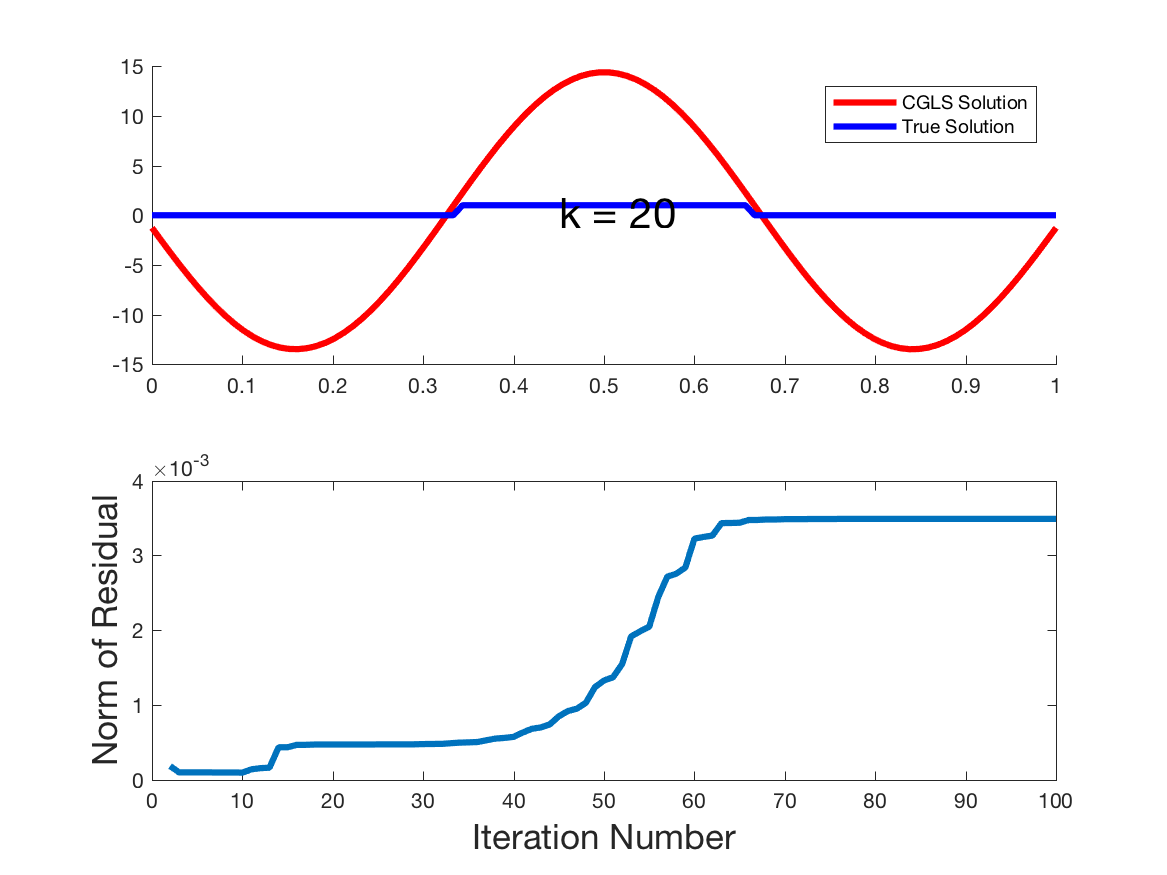
\includegraphics[height = 6 cm]{downsample_k20.png}
    }
    \caption{\label{fig:k20} CGLS Method for Reverse Heat Equation with only picking N/k points from the solution.}
\end{figure}

And here we pick 5 random points from the iteration to solve the inverse problem.

\begin{figure}[H]
    \centerline{
    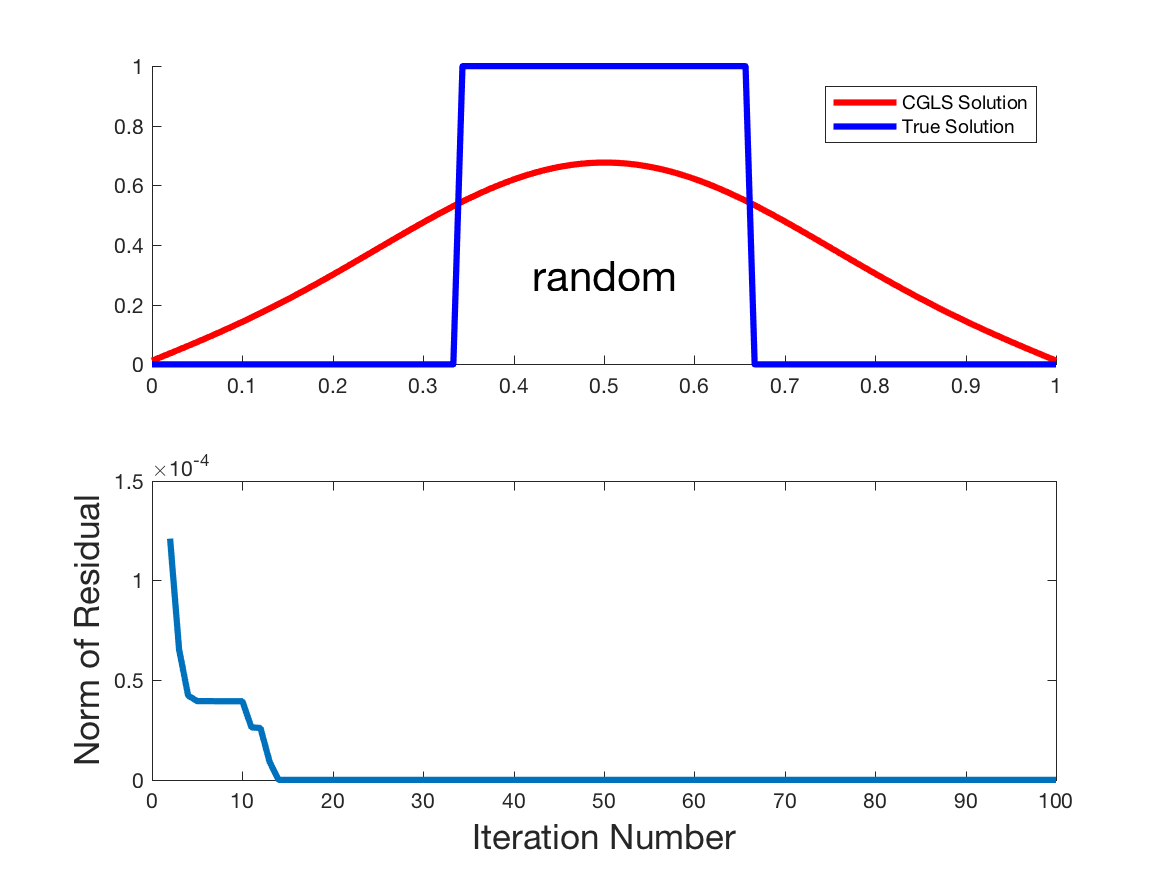
\includegraphics[height = 6 cm]{downsample_random.png}
    }
    \caption{\label{fig:random} CGLS Method for Reverse Heat Equation with only picking 5 random points from the solution.}
\end{figure}

Interestingly, the more points you pick, the worse the iteration seems to perform. The solution becomes larger in magnitude. This may be due to the fact that the actual solution only has two values (since it is a boxcar function) and it only needs a few points to be regularized.

The result does not indicate that the null space of the sparsely sampled forward matrix is a problem. It is because the solution does not have a lot of complexity and works well for functions of the boxcar type. However, since we used a 2nd order difference operator in the heat equation itself, we do see smoothness in the solution, which we would expect. We could test it without using the operator and see what the solution is like before regularizing.

\section{Appendix}

\subsection{CGLS Algorithms}

\subsubsection{\texttt{CGLS.m}}

\begin{verbatim}
    %%% This is the Conjugate Gradient Least Squares Algorithm, taken from
    %%% Erkki Somersalo's Notes. It solves the normal equations A'*A*x = A'*b.

    function [norms,x] = CGLS(A,b,noise)

        [~,n] = size(A);
        x = zeros(n,1);
        d = b; % Discrepancy Vector, for start, it is b because b - A(0) = b;
        r = A'*b; % residual error A'b - A'Ax = A'(b - Ax) = A'(b - A(0)) = A'b;
        p = r; % Search Directions
        t = A*p; % To save the matrix multiplication so we don't do it again.
        j = 1; % Iteration Variable
        MAXITER = 1000; % Max number of iterations to be safe
        tau = 1.2; % Safety Factor
        norms = zeros(MAXITER,1);
        norms(1) = Inf;

        while(norms(j) > tau*noise && j < MAXITER)

            alpha = (r'*r)/(t'*t);
            x = x + alpha*p;
            d = d - alpha*t;
            rnew = A'*d; % Matrix Multiplication #1
            beta = (rnew'*rnew)/(r'*r);
            p = rnew + beta*p;
            t = A*p; % Matrix Multiplication #2
            r = rnew;
            j = j + 1;
            norms(j) = norm(d);
        end

    end
\end{verbatim}


\subsubsection{\texttt{CGLSHeat.m}}
This is for the Heat Equation.
\begin{verbatim}
    %%% This is the Conjugate Gradient Least Squares Algorithm, taken from
    %%% Erkki Somersalo's Notes. It solves the normal equations A'*A*x = A'*b.


    %%% n is the size of discretization
    %%% b is the initial value
    %%% noise is the magnitude of noise we wish to use
    function [norms,x] = CGLSHeat(n,b,tspan,noise)
        % Heat equation by method of lines

        h = 1/n;
        D = 0.1; % Heat diffusion coefficient
        aux = zeros(n,1);
        aux(1) = -2;
        aux(2) = 1;
        L = toeplitz(aux);

        rhs = @(t,u) (D/h^2)*(L*u);

        x = zeros(n,1);
        d = b; % Discrepancy Vector, for start, it is b because b - A(0) = b;
        % r = A'*b; % residual error A'b - A'Ax = A'(b - Ax) = A'(b - A(0)) = A'b;
        [~,r] = ode15s(rhs,tspan,b);
        r = r(end,:)';
        p = r; % Search Directions
        % t = A*p; % To save the matrix multiplication so we don't do it again.
        [~, t] = ode15s(rhs,tspan,p);
        t = t(end,:)';
        j = 1; % Iteration Variable
        MAXITER = 100; % Max number of iterations to be safe
        tau = 1.2; % Safety Factor
        norms = zeros(MAXITER,1);
        norms(1) = Inf;

        while(norms(j) > tau*noise && j < MAXITER)

            alpha = norm(r)^2/norm(t)^2;
            x = x + alpha*p;
            d = d - alpha*t;
            [~,rnew] = ode15s(rhs,tspan,d); % This is A'*d
            rnew = rnew(end,:)';
            beta = norm(rnew)^2/norm(r)^2;
            p = rnew + beta*p;
            [~, t] = ode15s(rhs,tspan,p); % A*p
            t = t(end,:)';
            r = rnew;
            j = j + 1;
            norms(j) = norm(d);
        end

    end
\end{verbatim}

\subsubsection{\texttt{CGLSHeatDown.m}}

\begin{verbatim}
    function [norms, x] = CGLSHeatDown(N,b,noise,P)

    h = 1/N;
    D = 0.1; % Heat diffusion coefficient
    aux = zeros(N,1);
    aux(1) = -2;
    aux(2) = 1;
    L = toeplitz(aux);
    rhs = @(t,u) (D/h^2)*(L*u);
    tspan = linspace(0, 1, N)';



    x = zeros(N,1);
    d = P*b; % Discrepancy Vector, for start, it is b because Pb - P*A(0) = Pb;
    % r = A'P'*b; % residual error A'P'b - A'P'Ax = A'P'(b - Ax) = A'P'(b - A(0)) = A'P'b;
    [~,r] = ode15s(rhs,tspan,P'*d);
    r = r(end,:)';
    p = r; % Search Directions
    % t = PA*p; % To save the matrix multiplication so we don't do it again.
    [~, t] = ode15s(rhs,tspan,p);
    t = t(end,:)'; t = P*t;
    j = 1; % Iteration Variable
    MAXITER = 100; % Max number of iterations to be safe
    tau = 1.2; % Safety Factor
    norms = zeros(MAXITER,1);
    norms(1) = Inf;

    while(norms(j) > tau*noise*norm(b) && j < MAXITER)

        alpha = norm(r)^2/norm(t)^2;
        x = x + alpha*p;
        d = d - alpha*t;

        [~,rnew] = ode15s(rhs,tspan,P'*d); rnew = rnew(end,:)'; % This is A'*d
        beta = norm(rnew)^2/norm(r)^2;
        p = rnew + beta*p;

        [~, t] = ode15s(rhs,tspan,p); t = t(end,:)'; % A*p
        t = P*t;
        r = rnew;
        j = j + 1;
        norms(j) = norm(d);
    end



    end
\end{verbatim}

\subsection{\texttt{PMatrix.m}}

This function calculates the matrix that downsizes a vector based on how big the size of the vector is and the factor by which you want to downsize the vector.

\begin{verbatim}

    function [P] = PMatrix(k,N)
    %   k = number of points to skip for new discretization
    %   N = original discretization

    % First start off with the identity: discretization does not change

    P = eye(N);
    % Now, we find the number of points we can get.
    points = k:k:N;
    P = P(points,:);

    end


\end{verbatim}

\end{document}
